\documentclass{article}

\usepackage[a4paper, total={6in, 10in}]{geometry}
\usepackage[T2A]{fontenc}
\usepackage[utf8x]{inputenc}
\usepackage[english,russian]{babel}
\usepackage{graphicx}
\usepackage{float}
\usepackage{wrapfig}
\usepackage{hyperref}

\begin{document}

\begin{titlepage}
    \begin{center}
        \vspace*{5cm}

        \textbf{Линейные классификаторы и градиентные методы обучения}
    
        \vspace{0.5cm}
 
        \textbf{Сорокин Олег, 317}
 
        \vfill
             
        \vspace{0.8cm}
      
             
        каф. ММП, ВМК МГУ\\
        14.11.2022
             
    \end{center}
 \end{titlepage}

\newpage
\tableofcontents{}
\newpage

\section{Введение}
    В качестве первого приближения решения задач бинарной классификации часто рассматриваются линейные классификаторы. Этот класс методов основан на предположении о выполнении в данном датасете гипотезы линейной сепарабельности. Линейные классификаторы часто рекомендуются к применению в случае разреженности входной матрицы объектов-признаков. Далее рассмотрим одну из таких задач, а именно - определение токсичности комментария на основании матрицы встречаемости слов.

    Рассматривая датасет соответствующий этой задаче:
    \begin{itemize}
        \item Реализуем на языке Python с помощью библиотек numpy и scipy линейный классификатор, а также градиентный спуск (в т.ч. стохастический) с подсчётом необходимых величин (градиента, функционалов в точке и т.д.).
        \item Исследуем сходимость градиентного спуска и влияние этого процесса на качество модели в зависимости от гиперпараметров обучения.
        \item Проанализируем классические подходы к предобработке для увеличения качества текстовых моделей.
        \item Реализуем некоторые дополнительные методы, потенциально способные повысить качество модели.
    \end{itemize}

\section{Пояснения к задаче}
    При проведении экспериментов, в том числе при реализации метода градиентного спуска, будем пользоваться теоретическими выводами, описанными в этом разделе.

    Для начала дадим краткое описание линейной модели бинарной классификации, которую будем использовать. Пусть дана обучающая выборка $X = (x_i, y_i)_{i=1}^l$. Предположив, что множество объектов каждого из классов $y \in \{+1, -1\}$ отделено от другого некоторой гиперплоскостью, определим модель классификации как
    $$a_w(x) = sign(\langle w, x \rangle + w_0) = sign(\langle \hat{w}, \hat{x} \rangle),$$ где $\hat{w}$ - вектор параметров размерности на 1 большей, чем $w$, $\hat{x}$ - признаковое описание объектов с введённым константным ненулевым признаком.

    Критерием для обучения модели считаем минимизацию эмпирического риска, добиваться этого будем с помощью градиентного спуска. Получим явное выражение для градиента, чтобы ускорить процесс обучения и не прибегать к численным методам. Функционал качества с учётом $L2$-регуляризации с параметром силы регуляризации $\frac{\lambda}{2}$ запишем в виде
    \begin{equation} \label{eq:1}
        Q(X, w) = \frac{1}{l} \sum_{i=1}^{l}\mathcal{L}(M_i(w)) + \frac{\lambda}{2} ||w||^2_2
    \end{equation}
    где
    $$ M_i(w) = y_i * \langle w, x_i \rangle, $$
    $$ \mathcal{L}(M) = \log{(1 + \exp{(-M)})}$$
    Найдём дифференциал этого функционала:
    $$ d_wQ(X, w)[dw] = \frac{1}{l} \sum_{i=1}^{l}d\mathcal{L}(M_i) + \frac{\lambda}{2} d(||w||^2_2) = $$
    $$ = \frac{1}{l} \sum_{i=1}^{l}\frac{d(1 + \exp{(-M_i)})}{1 + \exp{(-M_i)}} + \frac{\lambda}{2} * 2||w||^2_2*d(||w||_2) = $$
    $$ = \frac{1}{l} \sum_{i=1}^{l}\frac{-\exp{(-M_i)}*d(M_i)}{1 + \exp{(-M_i)}} + \lambda||w||_2*d(\langle w, w \rangle^{1/2} ) = $$
    $$ = \frac{1}{l} \sum_{i=1}^{l}\frac{-\exp{(-M_i)}*y_i \langle x_i, dw \rangle}{1 + \exp{(-M_i)}} + \lambda||w||_2 * \frac{\langle w, dw \rangle}{||w||_2} = $$
    $$ = \langle \frac{1}{l} \sum_{i=1}^{l}(\frac{\exp{(-M_i)}}{1 + \exp{(-M_i)}} * (-y_i)) * x_i, dw \rangle +  \langle \lambda w, dw \rangle = $$
    $$ = \langle \lambda w - \frac{1}{l} \sum_{i=1}^{l}(\frac{1}{1 + \exp{(M_i)}} * y_i) * x_i, dw \rangle $$
    То есть
    \begin{equation} \label{eq:2}
        \nabla_w Q = \lambda w - \frac{1}{l} \sum_{i=1}^{l}(\frac{1}{1 + \exp{(M_i)}} * y_i) * x_i
    \end{equation}

    Теперь обобщим задачу на несколько классов. Пусть в той же постановке даны $K$ классов. Тогда вероятность каждого выразим как
    $$P(y=j | x) = \frac{\exp{(\langle w_j, x \rangle)}}{\sum_{k=1}^K\exp{(\langle w_k, x \rangle)}}$$
    Тем самым, задача сводится к методу максимального правдоподобия, то есть минимизации по всем весам для выражения
    $$Q(X, w) = -\frac{1}{l} \sum_{i=1}^llogP(y_i | x_i) + \frac{\lambda}{2} \sum_{k=1}^K||w_k||_2^2$$
    Для простоты в следующих выкладках положим $\lambda = 0$, то есть уберём регуляризацию. Рассмотрим один объект $x \in X$ класса $k \in K$ и по аналогии с бинарным случаем вычислим дифференциал, считая все веса, кроме некоторого $w_n$ фиксированными:
    $$d_{w_n}Q(x, w) = \frac{\sum_{i=1}^K \exp{(\langle w_i, x \rangle)}}{\exp{(\langle w_k, x \rangle)}} * \frac{\exp{(\langle w_n, x \rangle + \langle w_k, x \rangle) * d(\langle w_n, x \rangle) - [\sum_{i=1}^K \exp{(\langle w_i, x \rangle)}}] * d\exp{(\langle w_k, x \rangle)}}{(\sum_{i=1}^K \exp{(\langle w_i, x \rangle)})^2} = $$
    $$ = \frac{\exp{(\langle w_n, x \rangle) * d(\langle w_n, x \rangle) - [\sum_{i=1}^K \exp{(\langle w_i, x \rangle)}}] * d(\langle w_k, x \rangle)}{\sum_{i=1}^K \exp{(\langle w_i, x \rangle)}} = $$
    $$ = \langle \frac{\exp{(\langle w_n, x \rangle) * x - [\sum_{i=1}^K \exp{(\langle w_i, x \rangle)}}] * [n = k] * x}{\sum_{i=1}^K \exp{(\langle w_i, x \rangle)}}, dw_n \rangle = $$
    $$ = \langle (\frac{\exp{(\langle w_n, x \rangle)}}{\sum_{i=1}^K \exp{(\langle w_i, x \rangle)}} - [n=k]) * x, dw_n \rangle = $$
    \begin{equation} \label{eq:3}
        \nabla_{w_n}Q(x, w) = (\frac{\exp{(\langle w_n, x \rangle)}}{\sum_{i=1}^K \exp{(\langle w_i, x \rangle)}} - [n=k]) * x
    \end{equation}
    Суммируя по всем объектам выборки и учитывая слагаемое регуляризации, полученное в бинарном случае, выпишем искомое выражение
    \begin{equation} \label{eq:4}
        \nabla_{w_n}Q(X, w) = \lambda w_n-\frac{1}{l} \sum_{i=1}^l(\frac{\exp{(\langle w_n, x \rangle)}}{\sum_{i=1}^K \exp{(\langle w_i, x \rangle)}} - [n=y_i]) * x_i
    \end{equation}
    Теперь покажем, что (\ref{eq:2}) вытекает из (\ref{eq:4}) при рассмотрении двух классов $\{-1, +1\}$. Для этого без ограничения общности в (\ref{eq:3}) положим $n=+1$, рассматривая один объект класса $y$:
    $$(\frac{\exp{(\langle w_{y}, x \rangle)}}{\exp{(\langle w_{+1}, x \rangle) + \exp{(\langle w_{-1}, x \rangle)}}} - [y=+1]) * x$$
    Рассмотрим случай $y = +1$, остальные случаи рассматриваются аналогично:
    $$(\frac{\exp{(\langle w_{+1}, x \rangle)}}{\exp{(\langle w_{+1}, x \rangle) + \exp{(\langle w_{-1}, x \rangle)}}} - 1) * x = $$
    $$ = -\frac{\exp{(\langle w_{-1}, x \rangle)}}{\exp{(\langle w_{+1}, x \rangle) + \exp{(\langle w_{-1}, x \rangle)}}} * x = $$
    $$ = -\frac{1}{1 + \exp{(\langle w_{+1} - w_{-1}, x \rangle)}} * x$$
    Обозначим разность $(w_{+1} - w{-1})$ как новый вектор весов $w$. Рассмотрев все случаи и просуммировав по выборке, приходим к обобщённой записи (\ref{eq:1}).

    \section{Эксперименты}
        \subsection{Описание экспериментальных данных и их предобработка}
            Данные взяты с соревнования Kaggle "Toxic Comment Classification Challenge" и представляют собой размеченные по признаку токсичности комментарии из английской Википедии.

            Перед проведением экспериментов во всех текстах:
            \begin{itemize}
                \item все символы приведены к нижнему регистру, убраны ведущие и конечные пробелы;
                \item символы, не являющиеся буквами и цифрами, заменены на пробелы.
            \end{itemize}

            После этого для датасета была построена разреженная матрица объектов-признаков (Bag of Words), причём для первых экспериментов были исключены языковые единицы, встречающиеся менее чем в 25 документах (комментариях).
        \subsection{Анализ и сравнение методов градиентного спуска}
            \subsubsection{Программная реализации методов}
                На основании формул (\ref{eq:1}) и выведенной формулы для градиента бинарного линейного классификатора (\ref{eq:2}) были реализованы векторизованные методы подсчёта функции и её градиента. Проверка работы функций сверялась с численным подсчётом градиента произвольного функционала (правая производная с шагом $1e^{-8}$).
                
                Также реализован градиентный спуск, удовлетворяющий заданному набору тестов и стохастический (minibatch) градиентный спуск. Для тестирования последнего была взята выборка из 100.000 точек на плоскости, разделимая по классам прямой $y = 0$. При этом точность на валидационной выборке (20\% от обучающей) на каждом из 5 измерений достигала 0.95 и выше.
            \subsubsection{Анализ влияния гиперпараметров на градиентный спуск}
                Итерационный процесс сдвига в направлении антиградиента $Q(X, w)$ (см. (\ref{eq:1})) осуществляется по правилу
                $$w^{(k+1)} = w^k - \eta_k * \nabla_wQ(X, w), $$ где
                $$\eta_k = \frac{\alpha}{k^{\beta}}$$
                Начальное приближение в экспериментах, не связанных с его влиянием на результат, определяется случайным равномерно распределённым на отрезке $[0, 1]$ вектором. Чтобы это приближение не влияло на исход при пересоздании объекта классификатора, каждый переинициализируем зерно генерации случайных чисел.

                Зафиксируем $\beta = 0$ для рассмотрения влияния параметра шага $\alpha$ (тем самым отключив "угасание" градиента с каждой последующей итерацией). На рис. \ref{fig:1} показаны результаты для величины функции ошибки. Видно, что при $\alpha <= 0.01$ сходимость очень медленная, функция практически не изменяется. При $\alpha \in \{0.1, 1.0\}$ сходимость значительно быстрее. Шаг $\alpha = 10.0$ оказался слишком большим для попадания в точку минимума при заданной инициализации, что привело к расхождению метода. Эти замечания справедливы и для точности на валидационной выборке (рис. \ref{fig:2}). При $\alpha = 1.0$ на этом графике можем заметить колебания, что говорит о нестабильности процесса обучения.
                \begin{figure}[H]
                    \centering
                    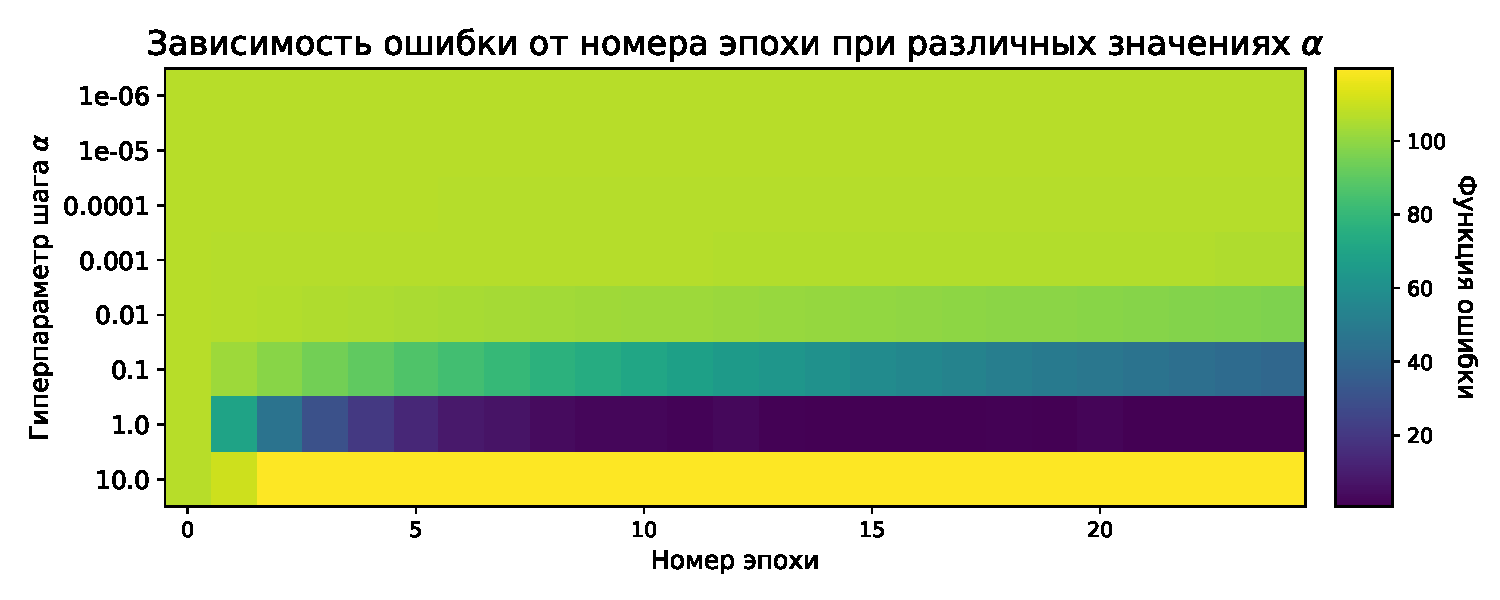
\includegraphics[width=0.8\linewidth]{./pictures/GDalphas_func.pdf}
                    \caption{Градиентный спуск: влияние $\alpha$ на ошибку в зависимости от итерации}
                    \label{fig:1}
                \end{figure}
                \begin{figure}[H]
                    \centering
                    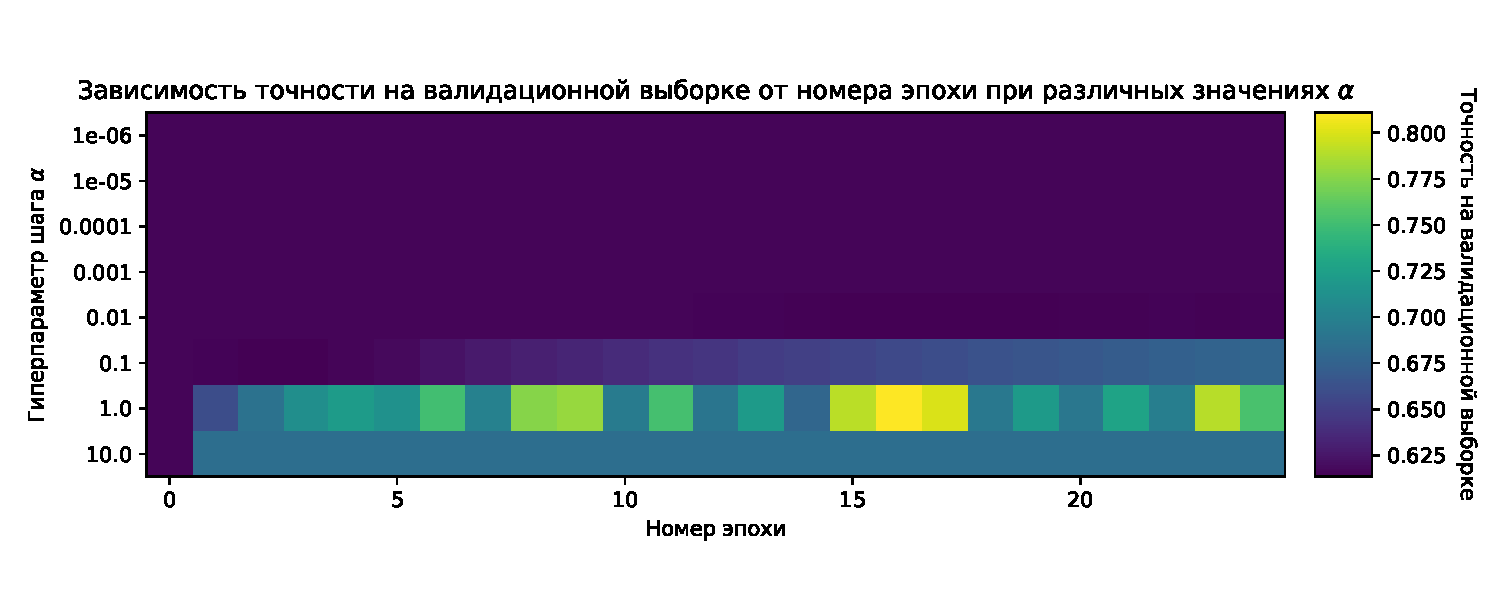
\includegraphics[width=0.8\linewidth]{./pictures/GDalphas_val_accuracy.pdf}
                    \caption{Градиентный спуск: влияние $\alpha$ на точность на валидационной выборке в зависимости от итерации}
                    \label{fig:2}
                \end{figure}

                Для решения проблемы нестабильности обучения проанализируем влияние параметра "угасания" градиента $\beta$, что потенциально способствует остановке алгоритма в точке локального минимума и предотвращению выхода из соответствующей зоны выпуклости графика. Зафиксируем $\alpha = 1.0$, при котором наблюдались осцилляции. На рис. \ref{fig:3} и \ref{fig:4} видим общий характер зависимостей ошибки и точности на валидации соответственно:
                \begin{itemize}
                    \item при $\beta < 0.022$ наблюдаем колебания по точности, сравнимые с $\beta = 0$, то есть влияние параметра незначительно;
                    \item при больших $\beta$ (на графике такое поведение отражено последней строкой) градиент по норме близок к нулю, после некоторой итерации эффекта от обучения практически нет;
                    \item остальные $\beta$ сглаживают процесс обучения. В аппендиксе приведено более подробное рассмотрение этого диапазона с целью поиска оптимального значения для последующих экспериментов. 
                \end{itemize}
                \begin{figure}[H]
                    \centering
                    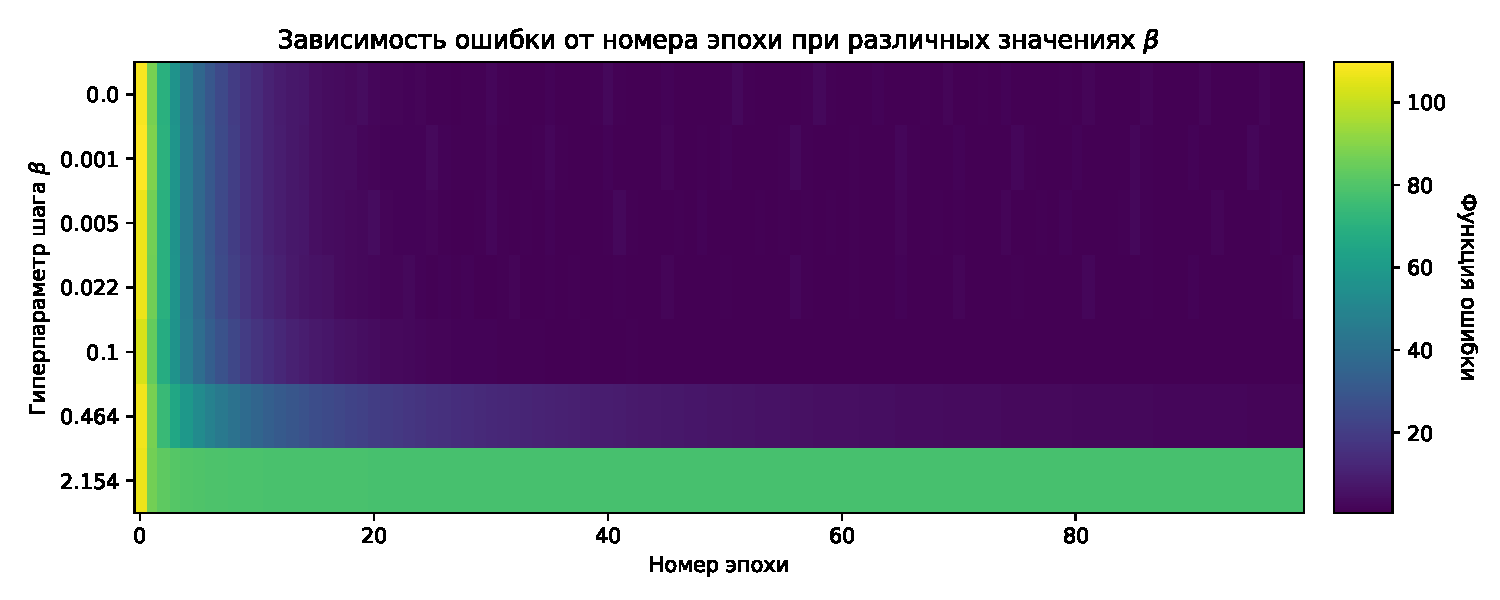
\includegraphics[width=0.8\linewidth]{./pictures/GDbetas_func.pdf}
                    \caption{Градиентный спуск: влияние $\beta$ на ошибку в зависимости от итерации}
                    \label{fig:3}
                \end{figure}
                \begin{figure}[H]
                    \centering
                    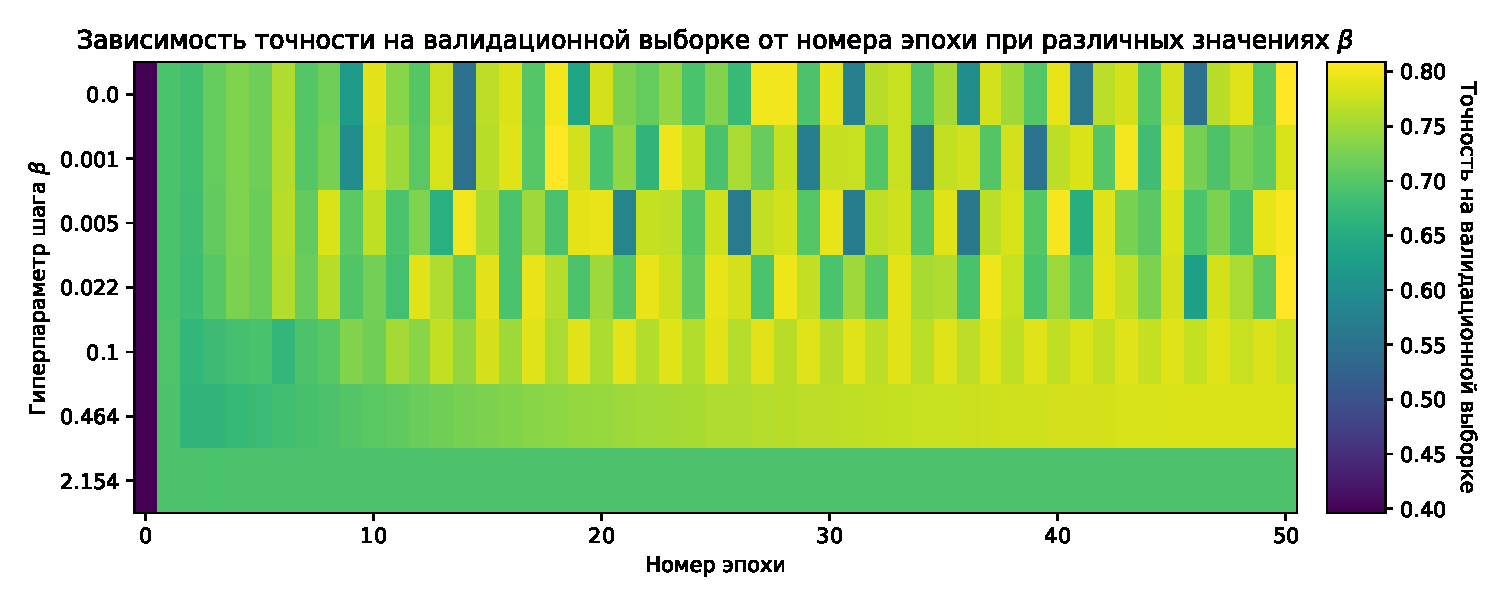
\includegraphics[width=0.8\linewidth]{./pictures/GDbetas_val_accuracy.pdf}
                    \caption{Градиентный спуск: влияние $\beta$ на точность на валидационной выборке в зависимости от итерации}
                    \label{fig:4}
                \end{figure}

                Наконец, при фиксированных оптимальных параметрах $\alpha = 1.0, \beta=0.3$ (см. аппендикс, рис. \ref{fig:11}, \ref{fig:12}) рассмотрим, как следующие стратегии инициализации влияют на исход:
                \begin{itemize}
                    \item нулевые веса;
                    \item единичные веса;
                    \item равномерные веса из отрезка $[0, 1]$;
                    \item равномерные веса из отрезка $[-5, 5]$;
                    \item нормально распределённые веса.
                \end{itemize}
                \begin{figure}[H]
                    \centering
                    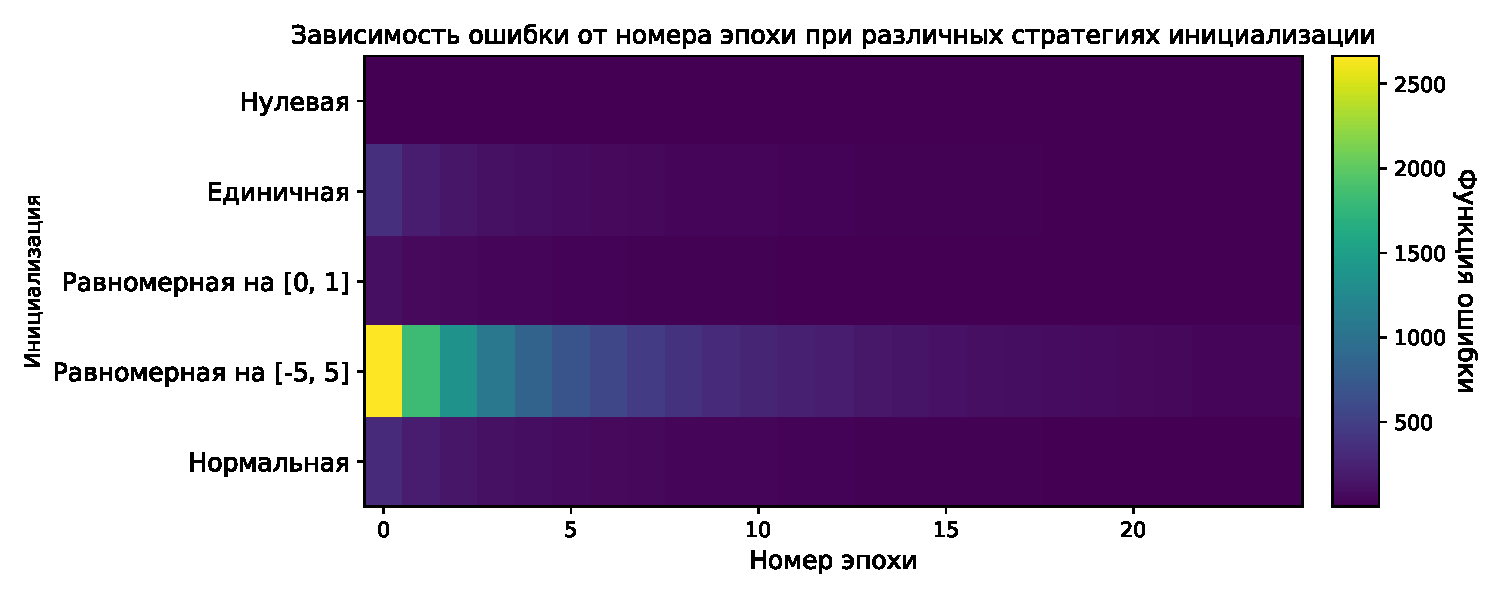
\includegraphics[width=0.8\linewidth]{./pictures/GDw0_func.pdf}
                    \caption{Градиентный спуск: влияние инициализации на ошибку в зависимости от итерации}
                    \label{fig:5}
                \end{figure}
                \begin{figure}[H]
                    \centering
                    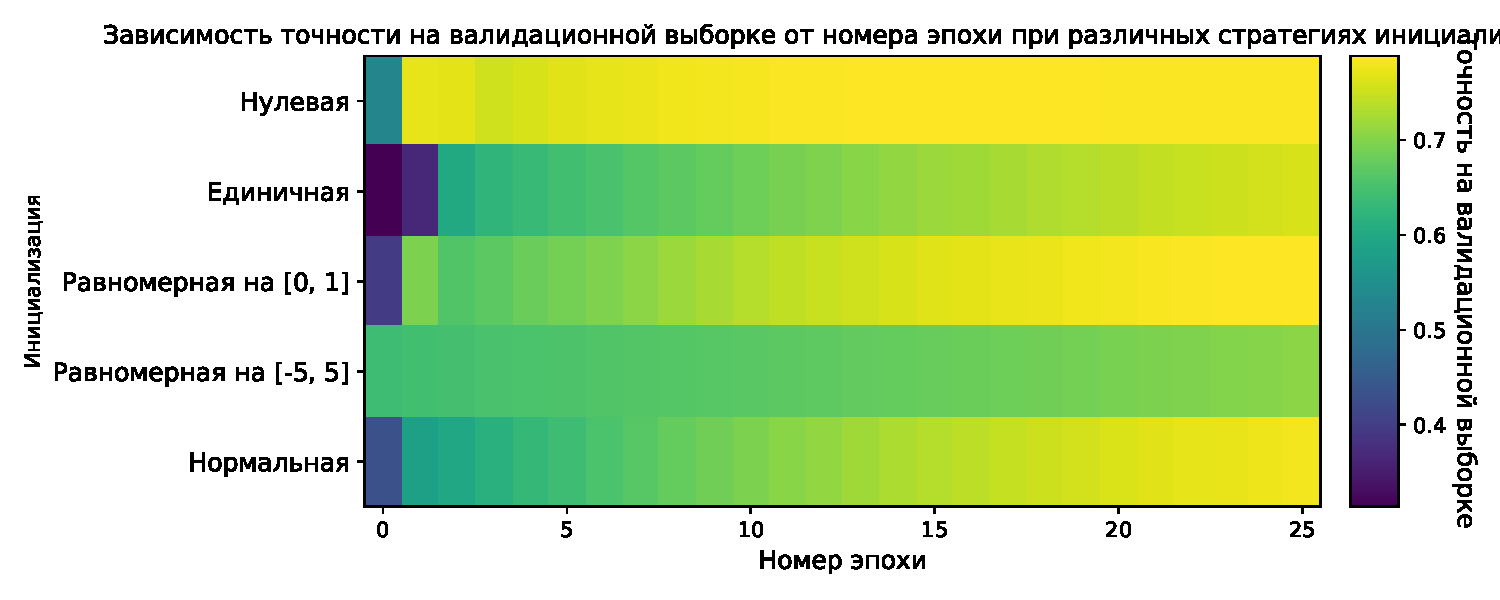
\includegraphics[width=0.8\linewidth]{./pictures/GDw0_val_accuracy.pdf}
                    \caption{Градиентный спуск: влияние инициализации на точность на валидационной выборке в зависимости от итерации}
                    \label{fig:6}
                \end{figure}
                На рис. \ref{fig:5}, \ref{fig:6} отражена динамика ошибки и точности на валидации соответственно.

                При нулевой инициализации после первой же итерации значения практически перестают меняться. Это связано с тем, что уже изначально многие бесполезные признаки были обнулены, а после первой итерации незначительно изменились наиболее полезные (рис. \ref{fig:7}).

                Для единичной и равномерной на [-5, 5] инициализаций характерен как наибольший пик на первой итерации, так и в целом наибольшие среди остальных изменения весов (рис. \ref{fig:7}). Это может означать, что соответствующие точки находятся дальше всего от искомой точки минимума.

                Оставшиеся две инициализации асимптотически совпадают с нулевой (как по ошибке, так и по точности на валидации).

                В дальнейших экспериментах будем использовать стандартную нормальную инициализацию.
                \begin{figure}[H]
                    \centering
                    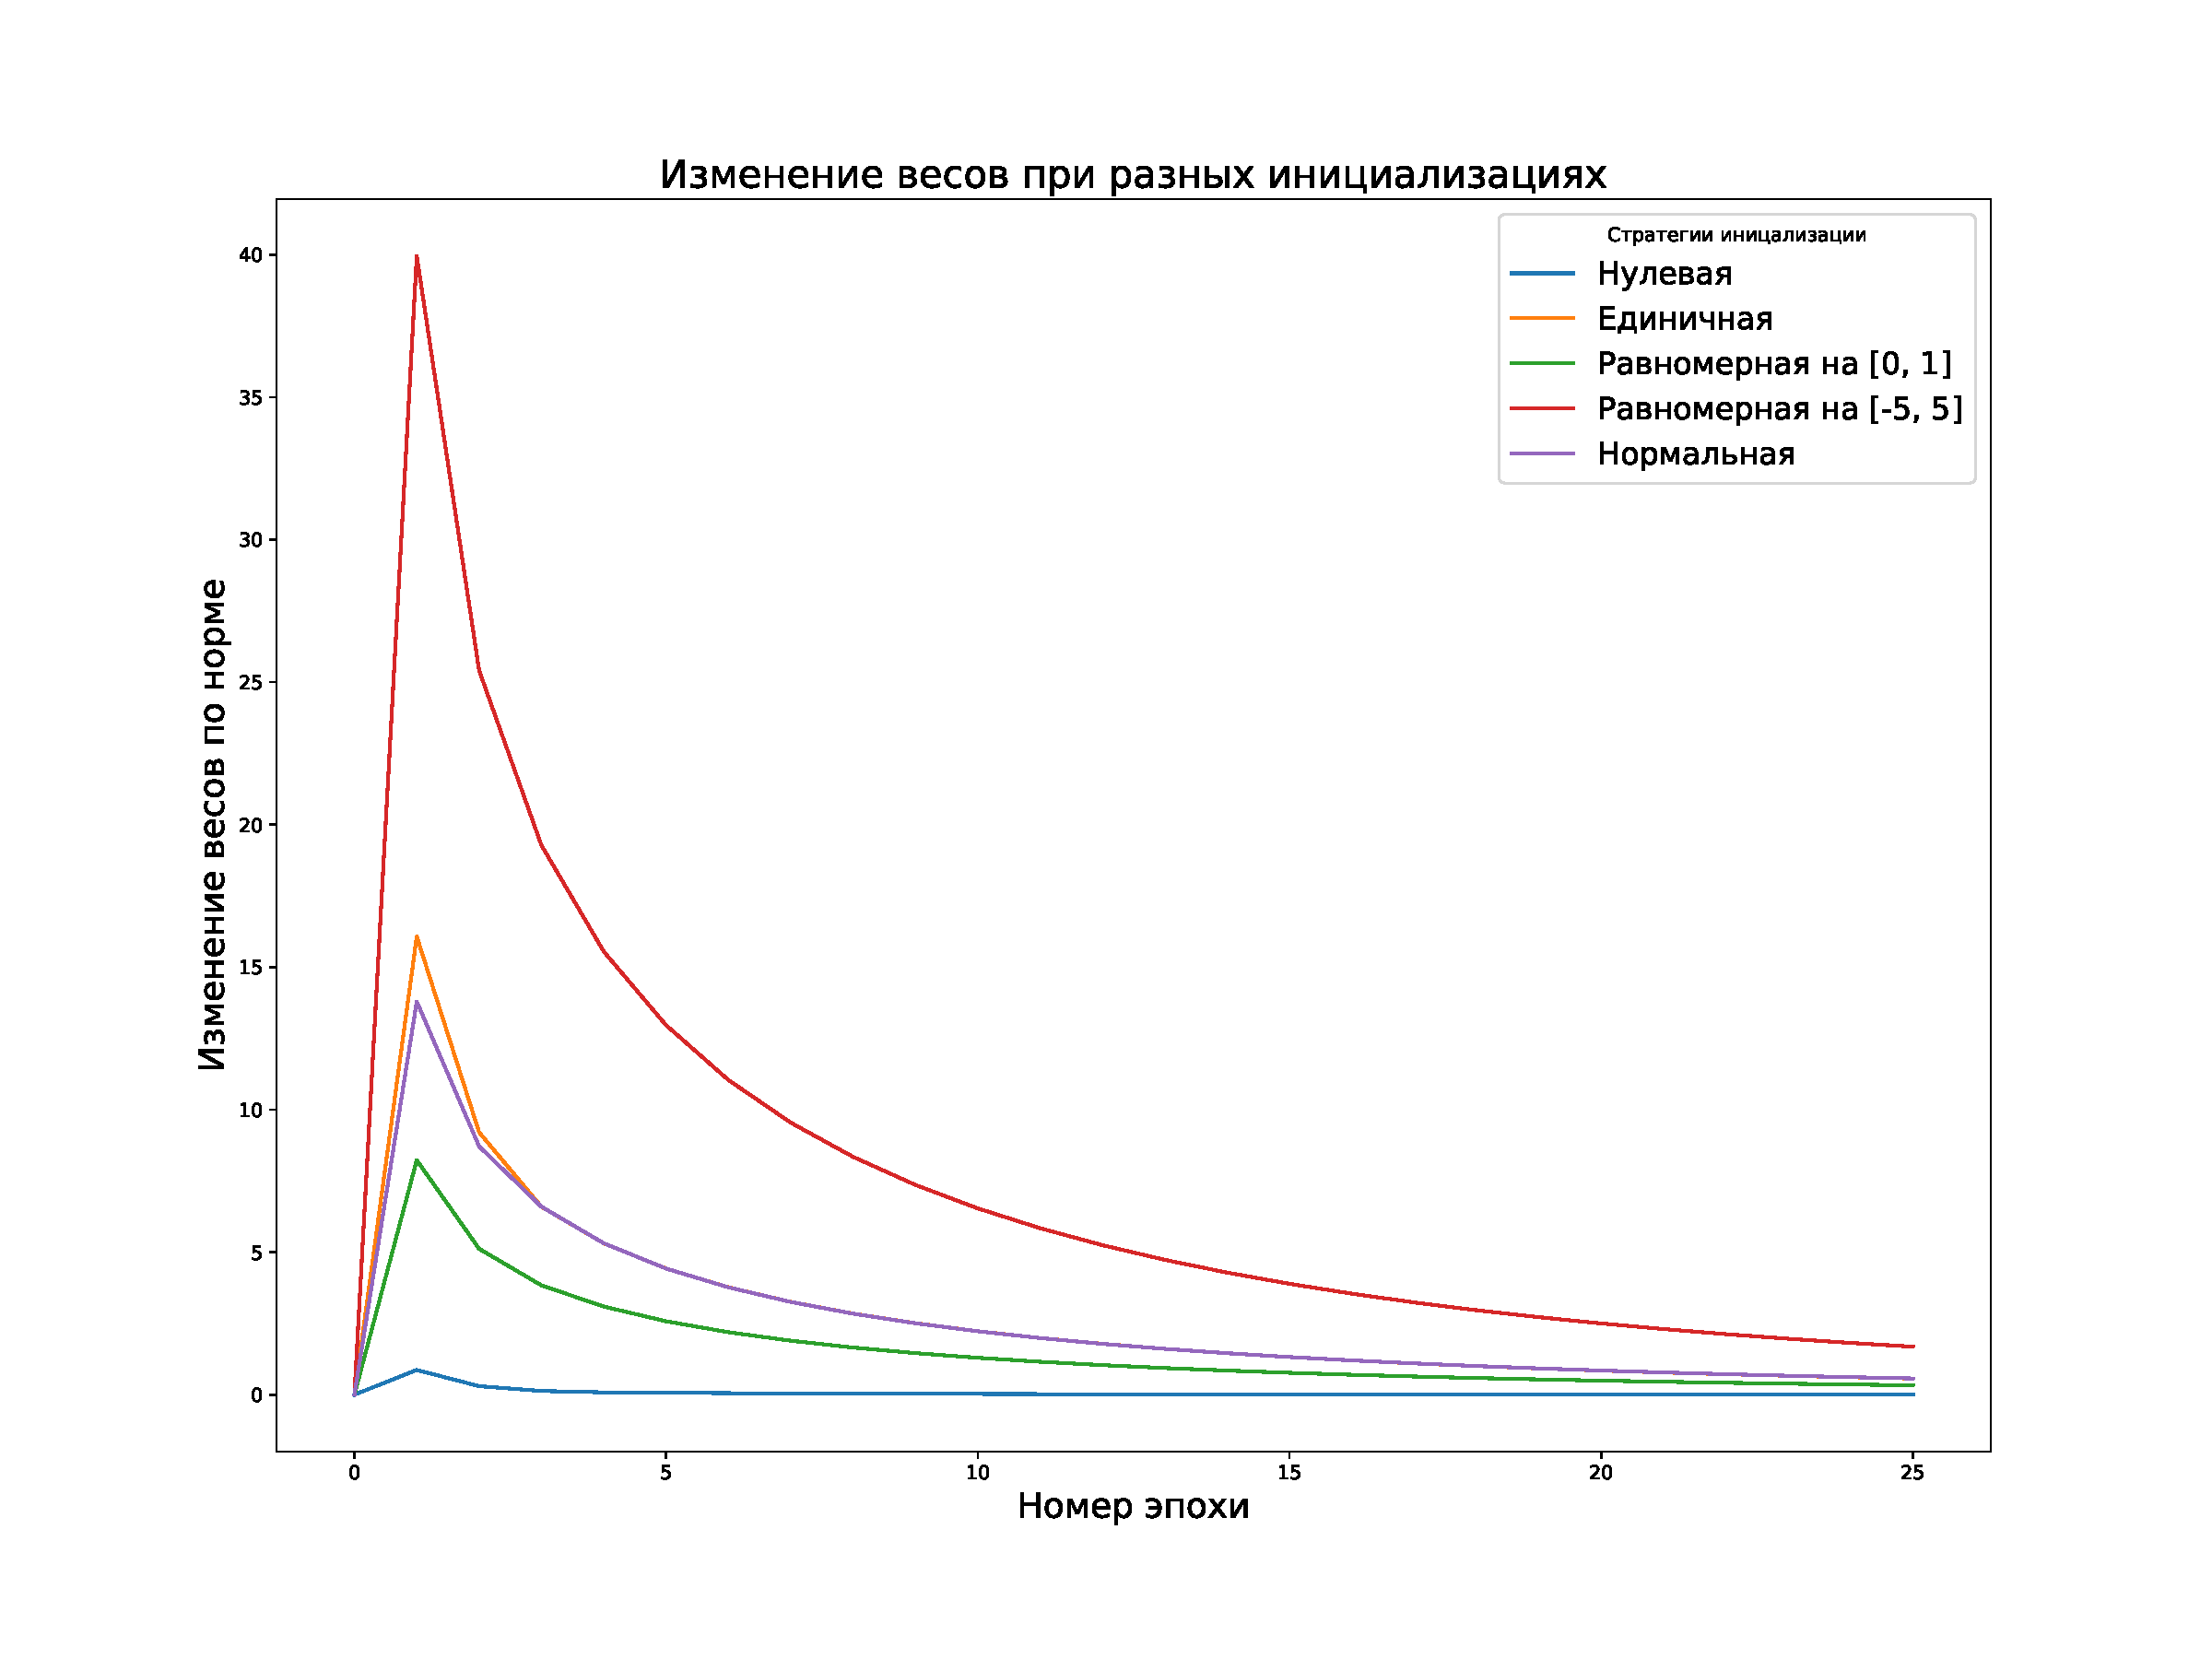
\includegraphics[width=0.8\linewidth]{./pictures/GDw0_w_diff.pdf}
                    \caption{Градиентный спуск: влияние инициализации на норму изменения весов на каждой итерации}
                    \label{fig:7}
                \end{figure}
            \subsubsection{Анализ влияния гиперпараметров на стохастический градиентный спуск, сравнение с градиентным спуском}
                Зафиксировав те же значения $\alpha = 1.0, \beta = 0.3$, рассмотрим поведение алгоритма при изменении размера батча (включая обычный градиентный спуск).
                
                Отметим, что некорректно сравнивать итерации при разных размерах батчей. Можно сравнивать целые эпохи, но чтобы собрать репрезентативную выборку о большом количестве проходов через весь датасет потребуется много времени. Вместо этого будем сравнивать алгоритмы по времени.

                \begin{figure}[H]
                    \centering
                    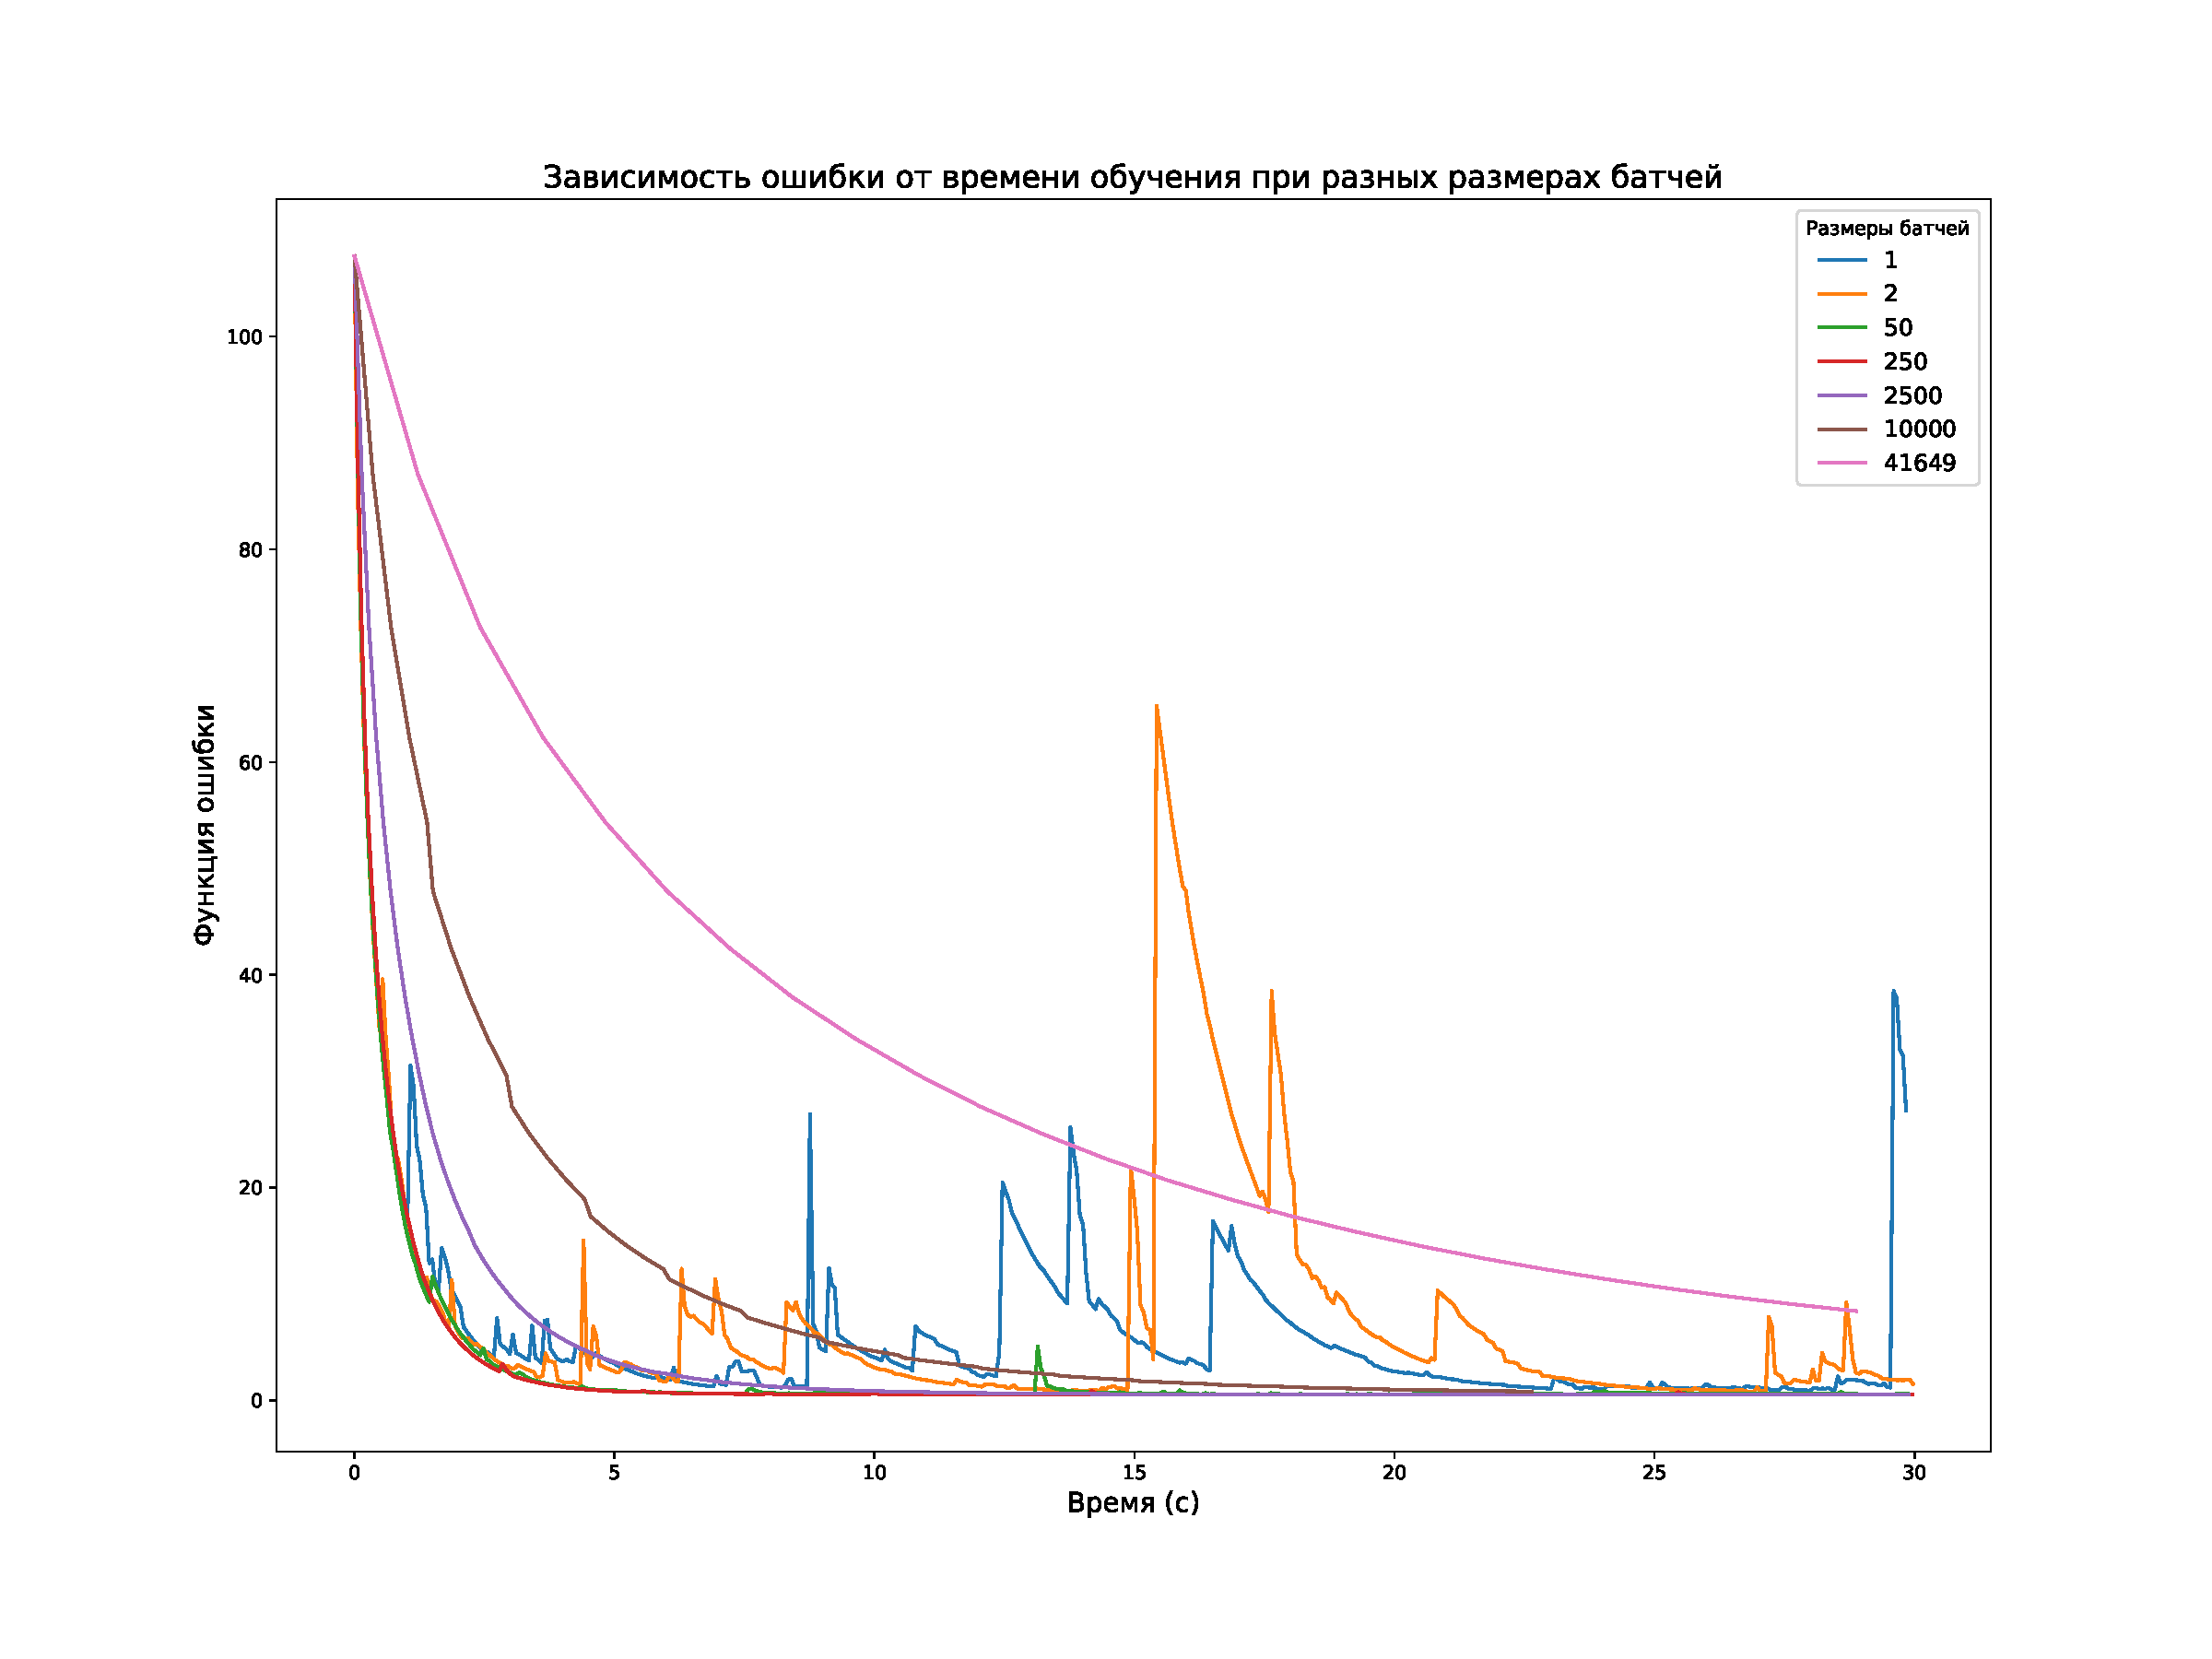
\includegraphics[width=0.8\linewidth]{./pictures/GDbatch_func.pdf}
                    \caption{Стохастический градиентный спуск: зависимость ошибки от времени }
                    \label{fig:8}
                \end{figure}
                На рис. \ref{fig:8} показано изменение ошибки по ходу обучения. Видно, что при градиентном спуске кривая обучения гладкая, но обучение при этом происходит очень медленно. С уменьшением размера батча графики становятся более ступенчатыми. Это связано с тем, что при итерации по батчам мы строим оценку градиента по всей выборке, которая может сильно отличаться (см. пики на рис. \ref{fig:8}) от правильного направления к оптимуму функции.
                \begin{figure}[t]
                    \centering
                    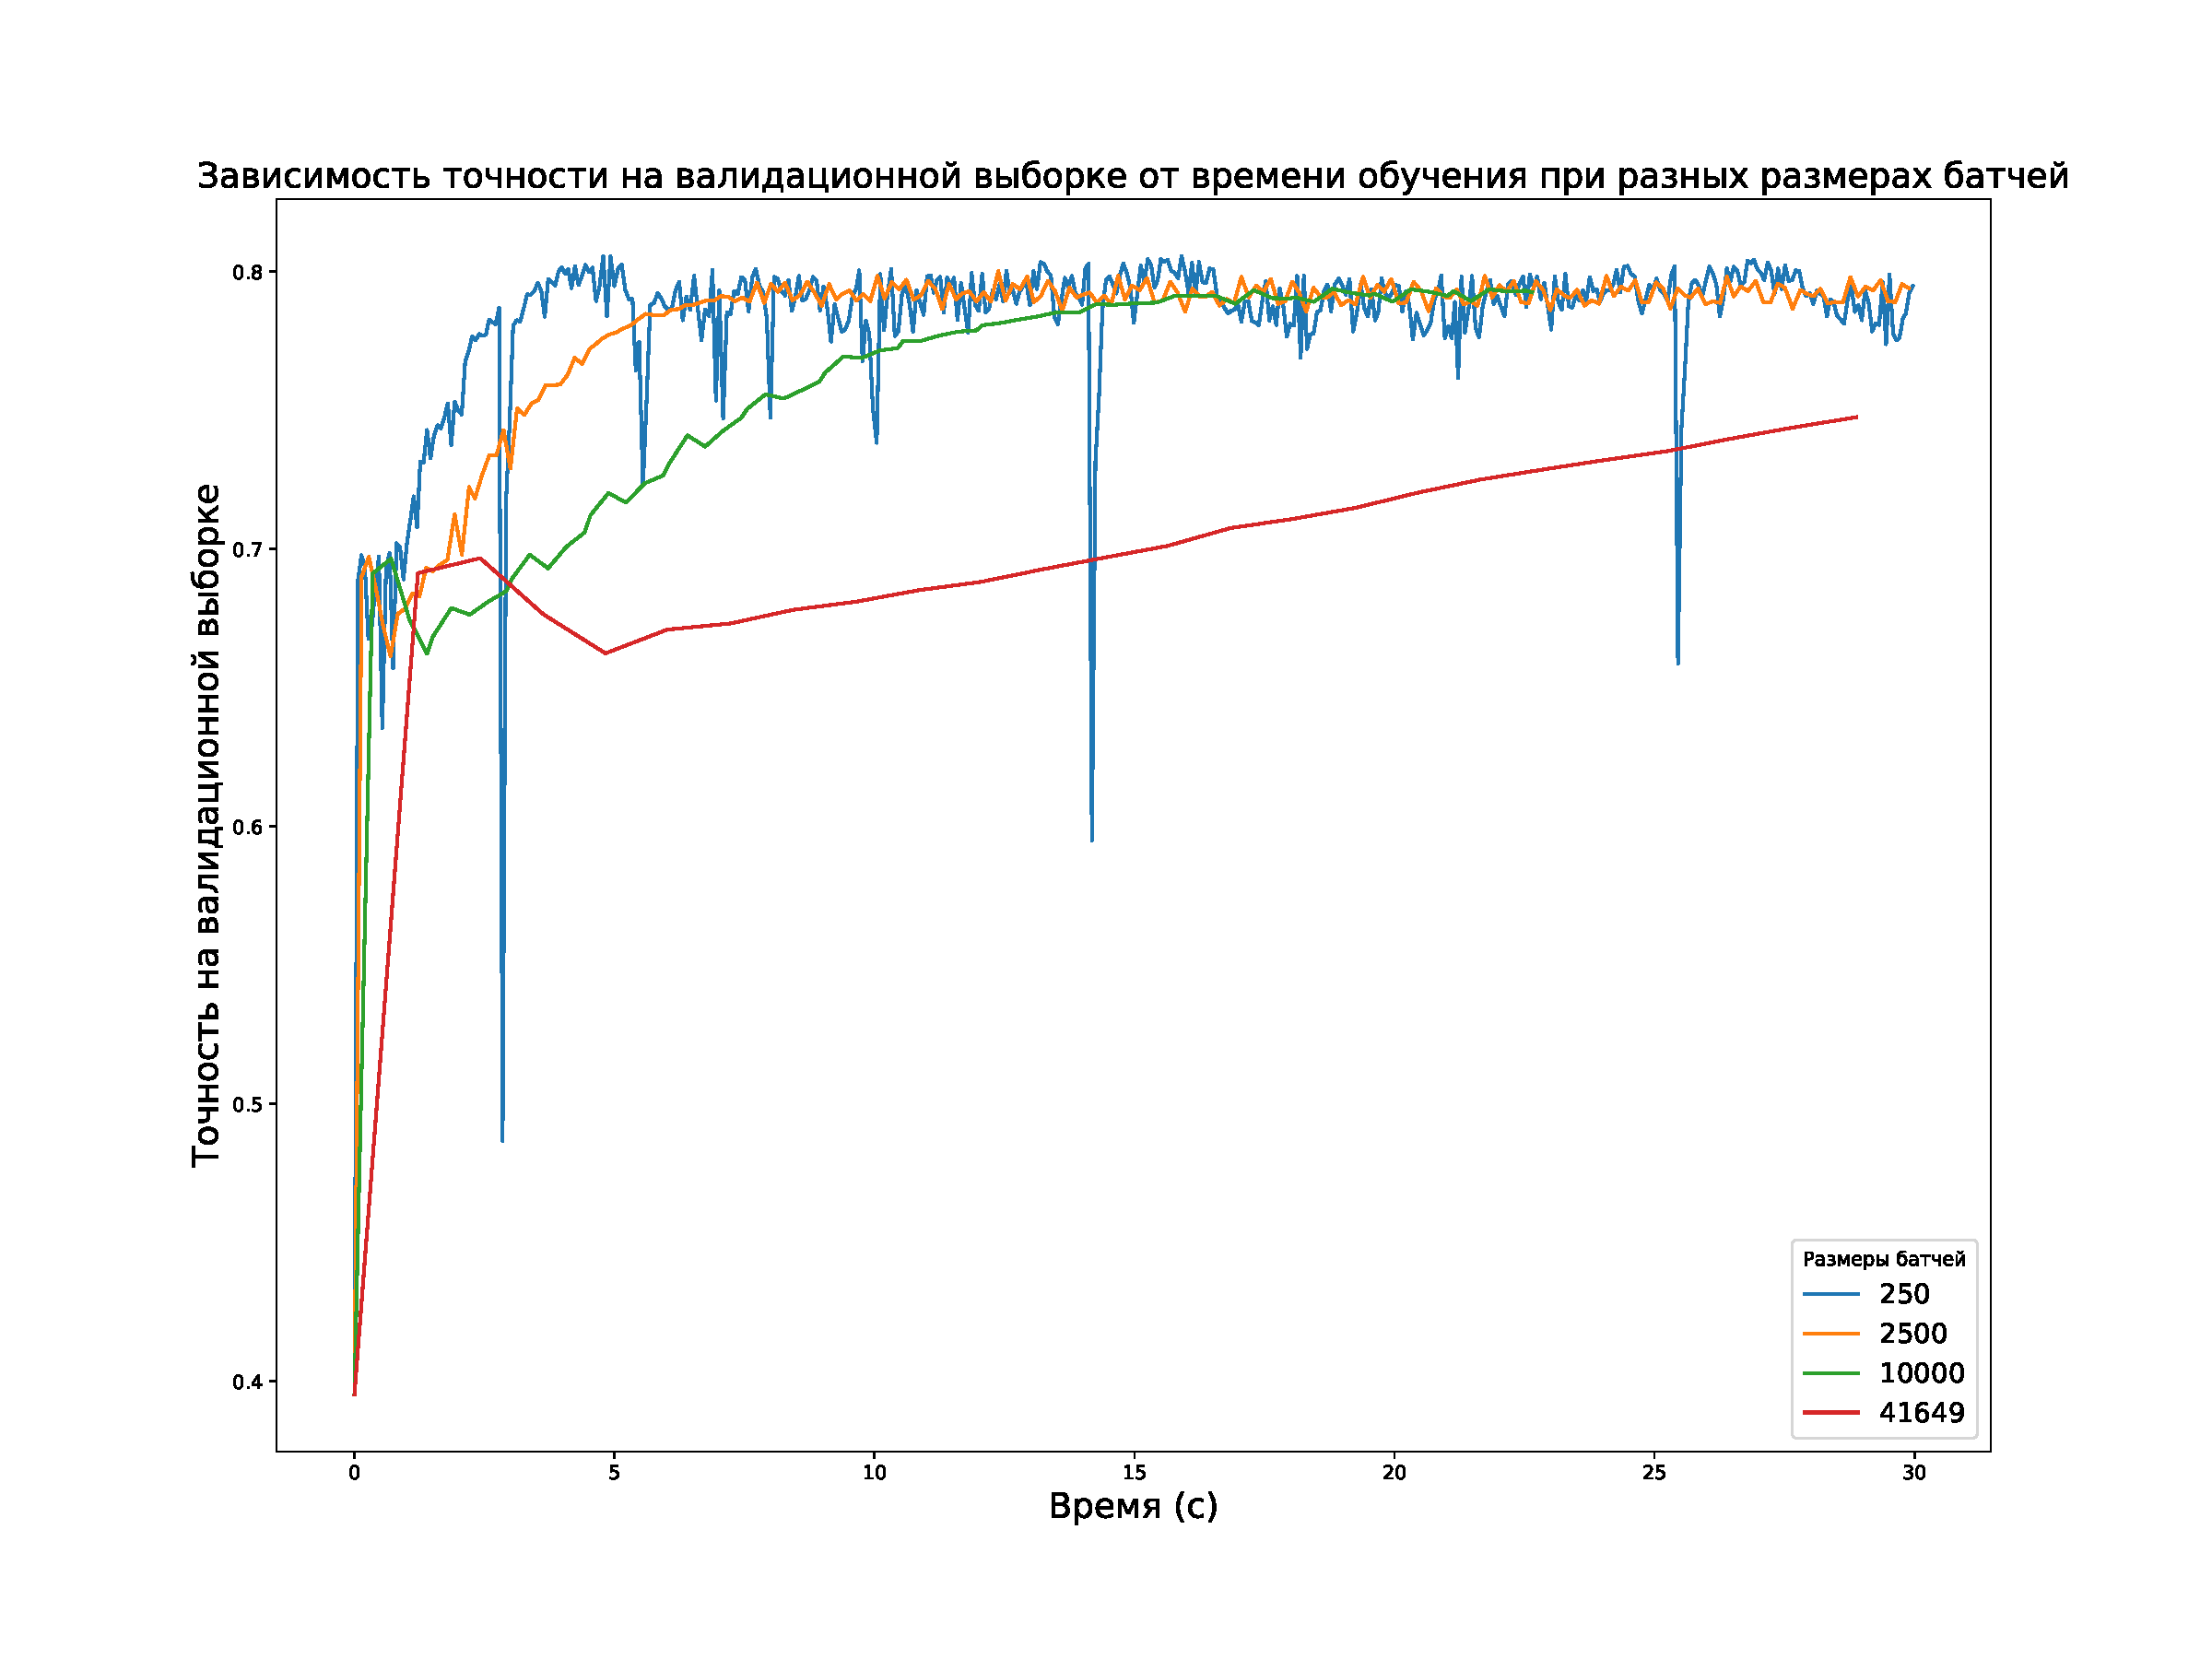
\includegraphics[width=0.8\linewidth]{./pictures/GDbatch_val_accuracy.pdf}
                    \caption{Стохастический градиентный спуск: влияние инициализации на точность на валидационной выборке в зависимости от итерации}
                    \label{fig:9}
                \end{figure}
                
                Рис. \ref{fig:9} отражает тот же смысл: оценка градиента может быть очень приблизительна, но скорость сходимости (имеется в виду сходимость в среднем) значительно возрастает. Некоторые графики могут быть очень шумными. Для данного рисунка соответствующие размеры батчей не учитывались.
                
                В ходе перезапуска аналогичных экспериментов с параметрами $\alpha, \beta$ для разных размеров батчей видны те же тенденции по эпохам, поэтому оптимальные параметры остаются теми же. Для примера ниже приведён график ошибки для батча размера 2500 (рис. \ref{fig:10}). В сравнении с рис. \ref{fig:1} вновь обнаруживаем, что при слишком малых значениях параметра обучение происходит слишком медленно, при больших значениях может возникнуть расходимость как на рис. \ref{fig:1} или осцилляция вокруг точки минимума, как на рис. \ref{fig:10}.
                \begin{figure}[H]
                    \centering
                    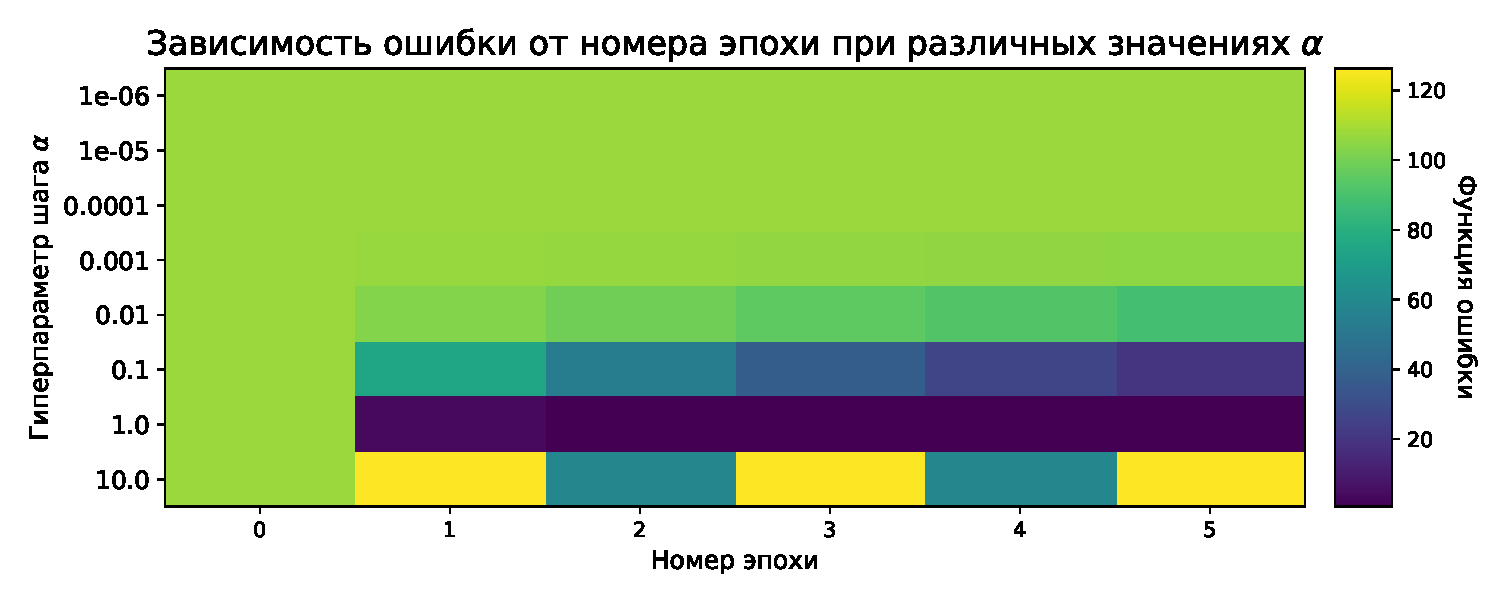
\includegraphics[width=0.8\linewidth]{./pictures/GDbatch2500_func.pdf}
                    \caption{Стохастический градиентный спуск: влияние параметра $\alpha$ на ошибку в зависимости от эпохи}
                    \label{fig:10}
                \end{figure}

                Таким образом, градиентный спуск и стохастический градиентный спуск имеют схожий смысл гиперпараметров (в том смысле, что динамика в обучении при их изменении сохраняется). Стохастический градиентный спуск по сравнению с обычной версией даёт значительный прирост по скорости работы алгоритма: оценивая градиент небольшим числом объектов можно быстро прийти в минимум. Эта оценка состоятельная, но при малой выборке может быть очень неточна и привести к движению в неправильном направлении.

            \subsubsection{Увеличение точности классификации, поиск наилучшего в этом смысле алгоритма}
                Зафиксируем те же параметры $\alpha, \beta, w_0$, используем батчи по 2500 объектов. Обучим алгоритм на 100 итерациях и посчитаем точность на тестовой выборке.

                Далее применим к обучающей выборке алгоритм лемматизации, то есть приведём словоформы к начальной форме. Такое преобразование позволит уменьшить размерность признакового пространства. Наконец, удалим из предложений стоп-слова. После применения каждого из этих алгоритмов пересчитаем точность.

                В таблицах ниже приведены результаты по применению алгоритмов и влиянию этого на точность на тестовой выборке, а также на время обучения алгоритма.

                CountVectorizer:
                \begin{center}
                    \begin{tabular}{| c | c | c | c |}
                        \hline
                        & Точность на тесте & Размерность & Время(с) \\
                        \hline
                        Без изменений & 0.738 & 6239 & 17.18\\
                        \hline
                        Лемматизация & 0.754 & 5167 & 12.98 \\
                        \hline
                        Лемматизация + удаление стоп-слов & 0.759 & 5042 & 12.31 \\
                        \hline
                    \end{tabular}
                \end{center}

                TfidfVectorizer (?!):
                \begin{center}
                    \begin{tabular}{| c | c | c | c |}
                        \hline
                        & Точность на тесте & Размерность & Время(с) \\
                        \hline
                        Без изменений & 0.698 & 6239 & 16.61\\
                        \hline
                        Лемматизация & 0.757 & 5167 & 13.07 \\
                        \hline
                        Лемматизация + удаление стоп-слов & 0.742 & 5042 & 11.89 \\
                        \hline
                    \end{tabular}
                \end{center}

                Так как наилучшую точность показал CountVectorizer (?!) с лемматизацией и удалёнными стоп-словами, далее работаем с этим представлением.

                Рассмотрим влияние параметра min\_df из конструктора CountVectorizer на точность на тестовой выборке, размерность признакового пространства и время работы:
                \begin{center}
                    \begin{tabular}{| c | c | c | c |}
                        \hline
                        min\_df & Точность на тесте & Размерность & Время(с) \\
                        \hline
                        3 & 0.737 & 21812 & 37.16\\
                        \hline
                        10 & 0.735 & 9128 & 12.98 \\
                        \hline
                        25 & 0.757 & 5042 & 12.31 \\
                        \hline
                        50 & 0.736 & 3170 & 8.68 \\
                        \hline
                    \end{tabular}
                \end{center}

                То есть изначально выбранный параметр min\_df = 25 близок к оптимальному.

                Из всех параметров модели остался неисследованным только коэффициент регуляризации. Изменение точности на тестовой выборке отражено в таблице:
                \begin{center}
                    \begin{tabular}{| c | c | c | c |}
                        \hline
                        L2 коэффициент & Точность на тесте \\
                        \hline
                        0.001 & 0.718 \\
                        \hline
                        0.01 & 0.729 \\
                        \hline
                        0.1 & 0.759 \\
                        \hline
                        1.0 & 0.743 \\
                        \hline
                        10.0 & 0.343 \\
                        \hline
                    \end{tabular}
                \end{center}

                То есть используемый ранее коэффициент регуляризации близок к оптимальному значению.

                Таким образом, лучший алгоритм в смысле точности на тестовой выборке описывается набором параметров:
                \begin{itemize}
                    \item $\alpha = 1.0, \beta=0.3$
                    \item $\lambda = 0.1$
                    \item batch\_size = 2500
                \end{itemize}

                Алгоритм чаще всего допускает ошибки в текстах, где токсичность проявляется в связи слов между собой. Например, если слова "europe", "hell", "genocide" по отдельности могут употребляться в повествовательном, нейтральном контексте, то вместе они могут давать токсичный политико-направленный эффект. Модель уловить эту связь не может (это сделать по набору слов невозможно и для человека) и часто помечает такие тексты как нетоксичные.

    \section{Дополнительные методы увеличения точности}
        \subsection{n\_grams для CountVectorizer}
            Поскольку CountVectorizer показал лучший результат (?!), n\_grams будем использовать применительно к нему. В таблице отражено влияние добавлений n\_gram в признаковое пространство. Начиная с $n=4$ наблюдается ухудшение качества, то есть становится слишком много неинформативных признаков.
            \begin{center}
                \begin{tabular}{| c | c | c |}
                    \hline
                    Макс. gram & Качество & Время(с) \\
                    \hline
                    1 & 0.757 & 12.31 \\
                    \hline
                    2 & 0.763 & 31.34 \\
                    \hline
                    3 & 0.765 & 40.64 \\
                    \hline
                    4 & 0.761 & 48.54 \\
                    \hline
                \end{tabular}
            \end{center}
        \subsection{PCA}
            -

    \section{Выводы}
            Модель линейного классификатора может быть полезна в задачах анализа текстов. Основная трудность в таких задачах - подбор парамеров предобработки текста для упрощения работы классификатора и гиперпараметров самой модели. Наиболее важными из таких гиперпараметров являются влияющие на шаг и "угасание" градиента параметры, а также параметр регуляризации. В зависимости от их значения алгоритм может как сойтись за несколько итераций, так и бесконечно осциллировать около точки минимума.

            Градиентный спуск позволяет подобрать веса для описанного классификатора с помощью сложновычислимого итерационного процесса. Стохастический градиентный спуск упрощает этот процесс: не нужно хранить огромные матрицы при итерации по батчам. Недостатком стохастического подхода является неточность оценки градиента.

            Модели такого типа плохо работают при больших размерностях признакового пространства. Существуют специальные методы уменьшения размерности матричных текстовых представлений (лемматизация, удаление стоп-слов), но могут оказаться полезными и общие методы (такие как PCA из utils).

            В случае анализа связанных текстов есть смысл добавить некоторые информативные признаки, иллюстрирующие эту связь. Примерами таких признаков являются n\_grams.

    \section{Аппендикс}
        \subsection{Графики для более точного подбора параметра $\beta$}
            \begin{figure}[H]
                \centering
                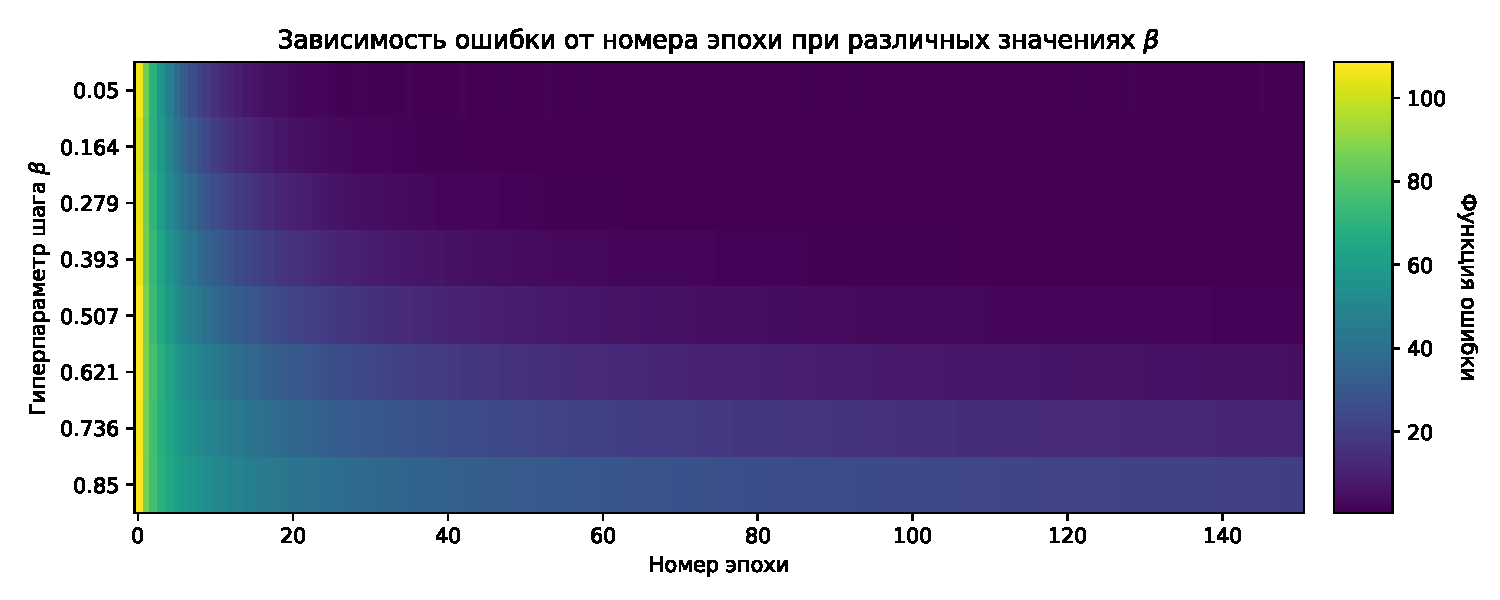
\includegraphics[width=0.8\linewidth]{./pictures/GDbetas_func2.pdf}
                \caption{Градиентный спуск: влияние $\beta$ на ошибку в зависимости от итерации}
                \label{fig:11}
            \end{figure}
            \begin{figure}[H]
                \centering
                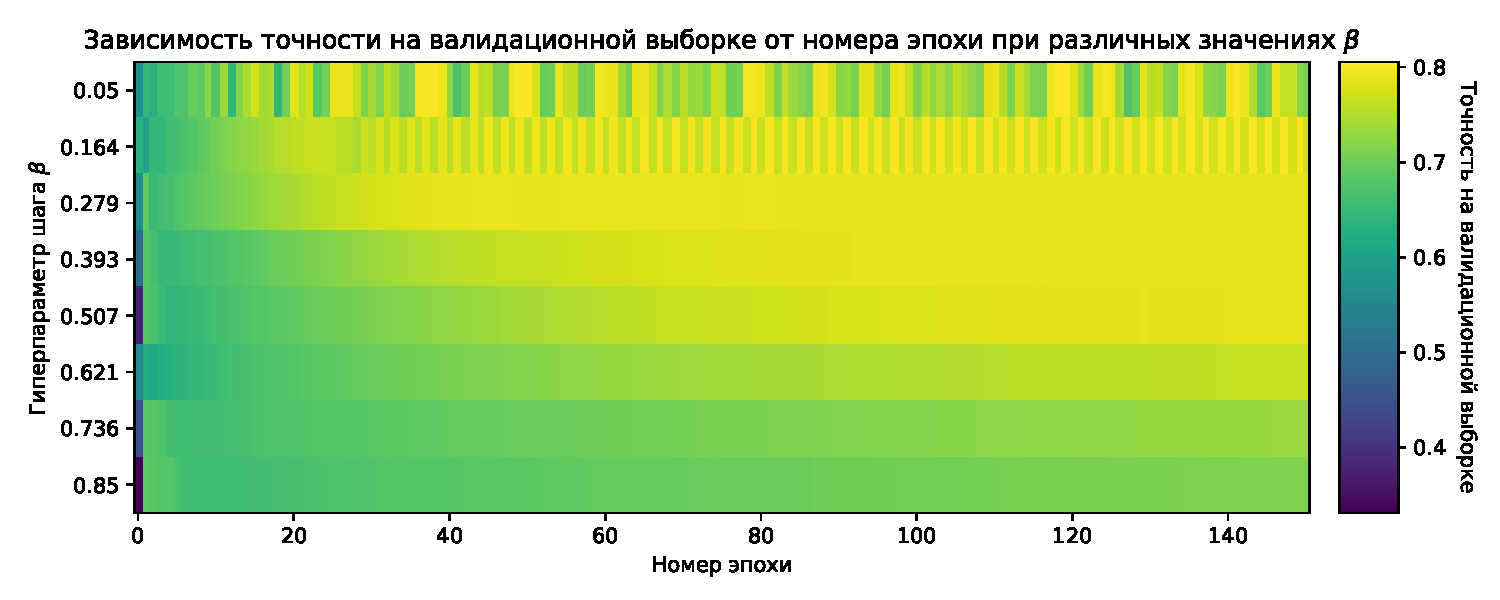
\includegraphics[width=0.8\linewidth]{./pictures/GDbetas_val_accuracy2.pdf}
                \caption{Градиентный спуск: влияние $\beta$ на точность на валидационной выборке в зависимости от итерации}
                \label{fig:12}
            \end{figure}


                
\end{document}